\documentclass{article}
\usepackage{graphicx}

\title{Cryptography}
\author{Rohan Dhillon}

\begin{document}

\maketitle
You have a message and you want to send it to a friend…but no one else can know about it. An age-old problem that has spurred a nuclear arms race to this day. Initially, the only way to achieve this was by walking, then horseback, then carrier pigeons, then the telegraph, then the telephone, and now, the internet. But someone can still “listen in” on the internet in the same way that someone can “guess” your password. How do they do it, and how do we protect ourselves?

The crux of modern cryptography relies upon this very important fact: big numbers are hard to factor. Take the number 3266999807178999181—I’m sure that if you saw that number on a math contest, your reaction would be “nope,” and even if you enlist a Java program to help you, it will still take a few minutes to get that the number only has two prime factors: 999999937 and 3267000013. 

So, why is this useful? Well, say we want to tell our agent to log into our Credit Suisse offshore account (obviously, we wouldn't want other people to know about this). We use a variation of “factoring numbers takes a long time” by using primitive roots modulo a prime p. An integer $g$ with $0<g<p$ is a primitive root if and only if $g^{p-1} \equiv 1 \pmod{p}$ and $g^k \not\equiv 1 \pmod{p}$ for all $0 < k < p-1$. 

\begin{center}
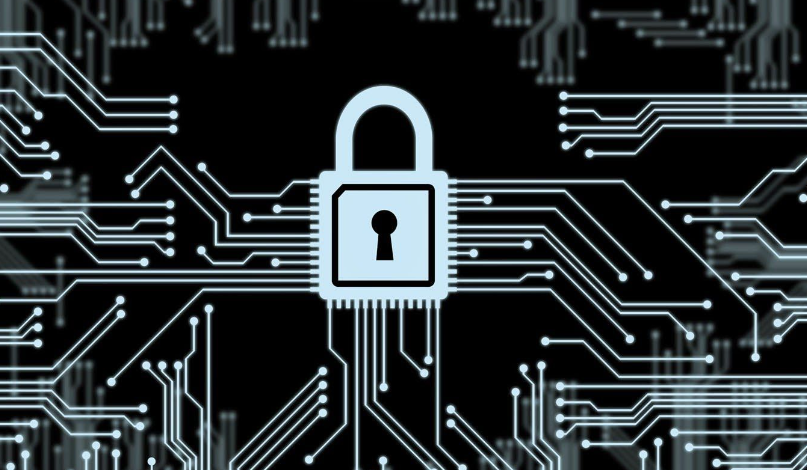
\includegraphics[scale=0.5]{images/crypto.png}
\end{center}

Both the agent and we decide to use the prime 11 as our modulo and $g=7$ as our primitive root. Both of these numbers are publicly available, but each of us has one number that is secret: we have $a=9$ and our agent has $b=4$. We can encrypt \textit{our} message by sending our agent $g^a \equiv 7^9 \equiv 8 \pmod{11},$ and our agent can send us $g^b \equiv 7^4 \equiv 3 \pmod{11}$ publicly. To decrypt the message, both of us take what we received to the power of our private key. We will get $3^9 \equiv 4 \pmod{11}$ and our agent will get $8^4 \equiv 4 \pmod{11},$ the same message! Intuitively, this makes sense as $g^{ba} \equiv g^{ab} \pmod{p}.$

Of course, this seems to not be \textit{that} useful since you both end up with a message, but this type of cryptography is usually used to set up a different, more efficient type called symmetric-key cryptography. As the name suggests, we both need the same key, but we don't want anyone else to know about it. And so both of us will start with two publicly known keys and then encrypt, exchange, and decrypt to get the same, now secret, key...now what?

We have the key 4, which is 100 in binary. Suppose we want to send the code 01101111 01110000 01100101 01101110, which corresponds to the word "open" using ASCII characters (each letter and typed symbol--not Unicode character--corresponds to a number between 0 and 128). In the simplest case, we can just use XOR encryption which returns a 1 if and only if the codes have different values at that position. Doing this yields a new code: 11111101 00111001 01000001 11111100, which we may send to our agent. They also have the key 100, and they can just apply the XOR function to the code they received to get the message: 01101111 01110000 01100101 01101110, "open."

And now our agent knows to open the offshore Credit Suisse account we've been storing our stock earnings in! Usually with this type of encryption and decryption, we would use \textit{giant} numbers with hundreds of digits to make sure that anyone trying to crack the code would have to wait until the death of the sun to do so. Interestingly, this is also why prime numbers are so important in our modern lives--there's even a book with random large primes that's on sale for \$60. After that not-at-all tax-evasionary article, I hope you walk away with a greater understanding of the real use mathematics has in our modern life--whenever you cry out "when will I ever use this in my life??" during math class, chances are you already have.
\end{document}